\section{Pneumatic System}

The goal of this section is to describe the design work completed for the pneumatic actuation system.

In Section \ref{sec:transmission_control_background} the background of the transmission and the control system used in previous years was discussed. The design of the transmission control scheme for this project therefore improves upon the previous generation by targetting several of the noted deficiencies, while reusing specific portions that worked well.

Sizeable consideration was made for replacing the pneumatic system with a fully electronic one. However, it was determined that the power to weight ratio of electric motors and gearboxes was far less than that of a pneumatic solution for the amount of torque required.

After deciding to not change away from pneumatics, an improved actuation scheme was proposed that would both improve the controllability and efficiency of the system. A diagram of the mechanical portion of the pneumatics system can be seen in Figure \ref{fig:pneumatics_design}. An on-board compressed air tank is fitted with a pressure regulator, which regulates the system pressure to approximately $120\,psi$. 4 electronically controlled pneumatic valves control the flow of air to and from 2 pneumatic actuators.

\subsection{Purpose}

Actuation of the clutch and gear selection levers. 

Be controlled electronically by the transmission control module.


\subsection{System Overview}

\begin{figure}
\centering
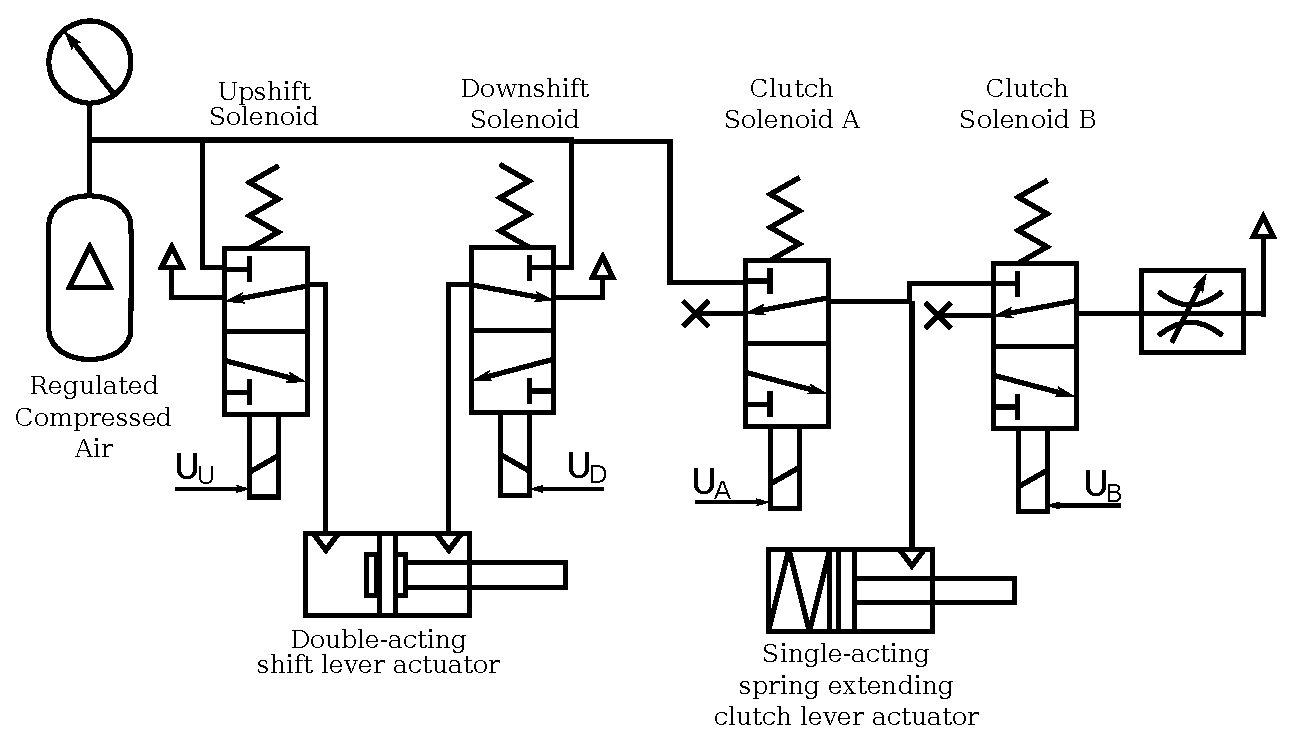
\includegraphics[scale=0.5]{design/figures/pneumatics}
\caption{Transmission control pneumatics design.}
\label{fig:pneumatics_design}
\end{figure}

\paragraph{Shift Actuator}

The first actuator, visible on the left of Figure \ref{fig:pneumatics_design}, actuates the shift lever between 3 different positions: upshift, downshift, and rest-state. The transmission spring-loads the lever to automatically return to the rest-state, which we have set up to be half-way through the actuator stroke. Individually applying pressure to one port will pull the lever up, and to the other port, down.

Current gear position is determined with a potentiometer that is mechanically linked to the shift drum. Control and timing are generated by the micro-controller, and respond to requests from the driver.

\paragraph{Clutch Actuation}

The second actuator, visible on the right of Figure \ref{fig:pneumatics_design}, actuates the clutch lever. Precise control of the clutch is accomplished with fast solenoid valves. The valves are signalled with a \emph{Pulse Width Modulated} (PWM) signal, which modulates the average mass air flow rate into and out of the cylinders. Position feedback for the clutch and shift levers is provided by magnetic sensing membrane potentiometers. 

\nomenclature{PWM}{Pulse Width Modulation}

The shift lever does not require the same level of control as the clutch, but utilizes the same hardware to facilitate the possibility of using a stock shifting drum without gear position feedback.

\begin{figure}[H]
	\centering
%		\input{Figures/transmission_system_overview}
	\caption{Transmission system overview.}
	\label{fig:transmission_system_overview}
\end{figure}

\subsubsection{Air tank}

An on-board compressed air tank 

\subsubsection{Regulator}

The air tank is fitted with a pressure regulator, which regulates the system pressure to approximately $120\,psi$. 

\subsubsection{Valves}

4 electronically controlled pneumatic valves control the flow of air to and from 2 pneumatic actuators.

\subsubsection{Cylinders}


\subsubsection{Mechanical Linkage }


\subsubsection{Positional Sensors }


\subsection{Valving Design}

Reduces air consumption

Increases controllability


\subsection{Modelling}

Entire system modelled in Simulink